\item \points{1a}

Please implement the following two baselines in ~submission.py~.
\begin{enumerate}
    \item \textit{Fixed-dose}: This approach will assign 35mg/week (medium) dose to all patients.
    \item \textit{Warfarin Clinical Dosing Algorithm}: This method is a linear model based on age, height, weight, race and medications that patient is taking. You can find details of the exact model below which is taken from section S1f of ~data/appx.pdf~.
\end{enumerate}

\begin{figure}[H]
\centering
  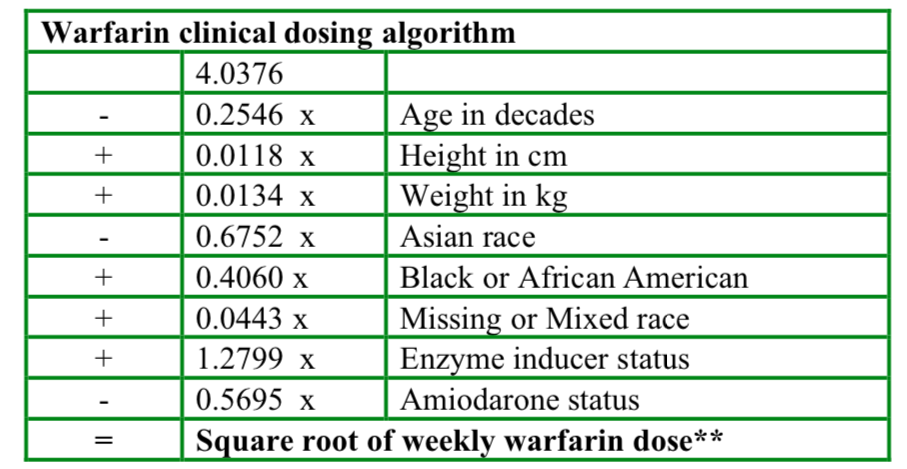
\includegraphics[width=.5\linewidth]{images/clinical_model.png}
  \caption{Definition of clinical (linear) model take from section 1f of appx.pdf}
\end{figure}

Run the fixed dosing algorithm and clinical dosing algorithm with the following commands respectively:

\begin{lstlisting}
$ python run.py --model fixed
$ python run.py --model clinical
\end{lstlisting}

You should see the total\_fraction\_correct to be fixed at about 0.61 for fixed dose and 0.64 for clinical dose algorithm.

\textit{Hint: Look into section 1f of appx.pdf for a description of the features used in the clincal model}
